\documentclass[11pt,a4paper]{article}
\usepackage[margin=2cm]{geometry}
\usepackage{hyperref}
\usepackage{times}
\usepackage{graphicx}
\usepackage{enumitem}
\setlist[itemize]{itemsep=2pt, topsep=2pt, parsep=0pt, partopsep=0pt}
\usepackage[none]{hyphenat}

\begin{document}

\begin{center}
\Large \textbf{Research Statement}\\
\vspace{0.2cm}
\normalsize Arman Asgharpoor\\
DPhil Application -- Autonomous Intelligent Machines and Systems\\
University of Oxford\\
Word count: 2,359
\end{center}

\vspace{0.3cm}


The reconstruction in Figure~\ref{fig:mesh} was built from this space: 
the Fasta Robotics lab, a barrel-vaulted office with glass partitions, 
rolling chairs, and an open testing area beyond. Five minutes of capture. 
The arch, the desks, the floor tiles are all there. What is not: that the 
glass rear wall is transparent, that the chairs will be elsewhere tomorrow, 
that the shape in the central aisle was a person.

\begin{figure}[h]
\centering
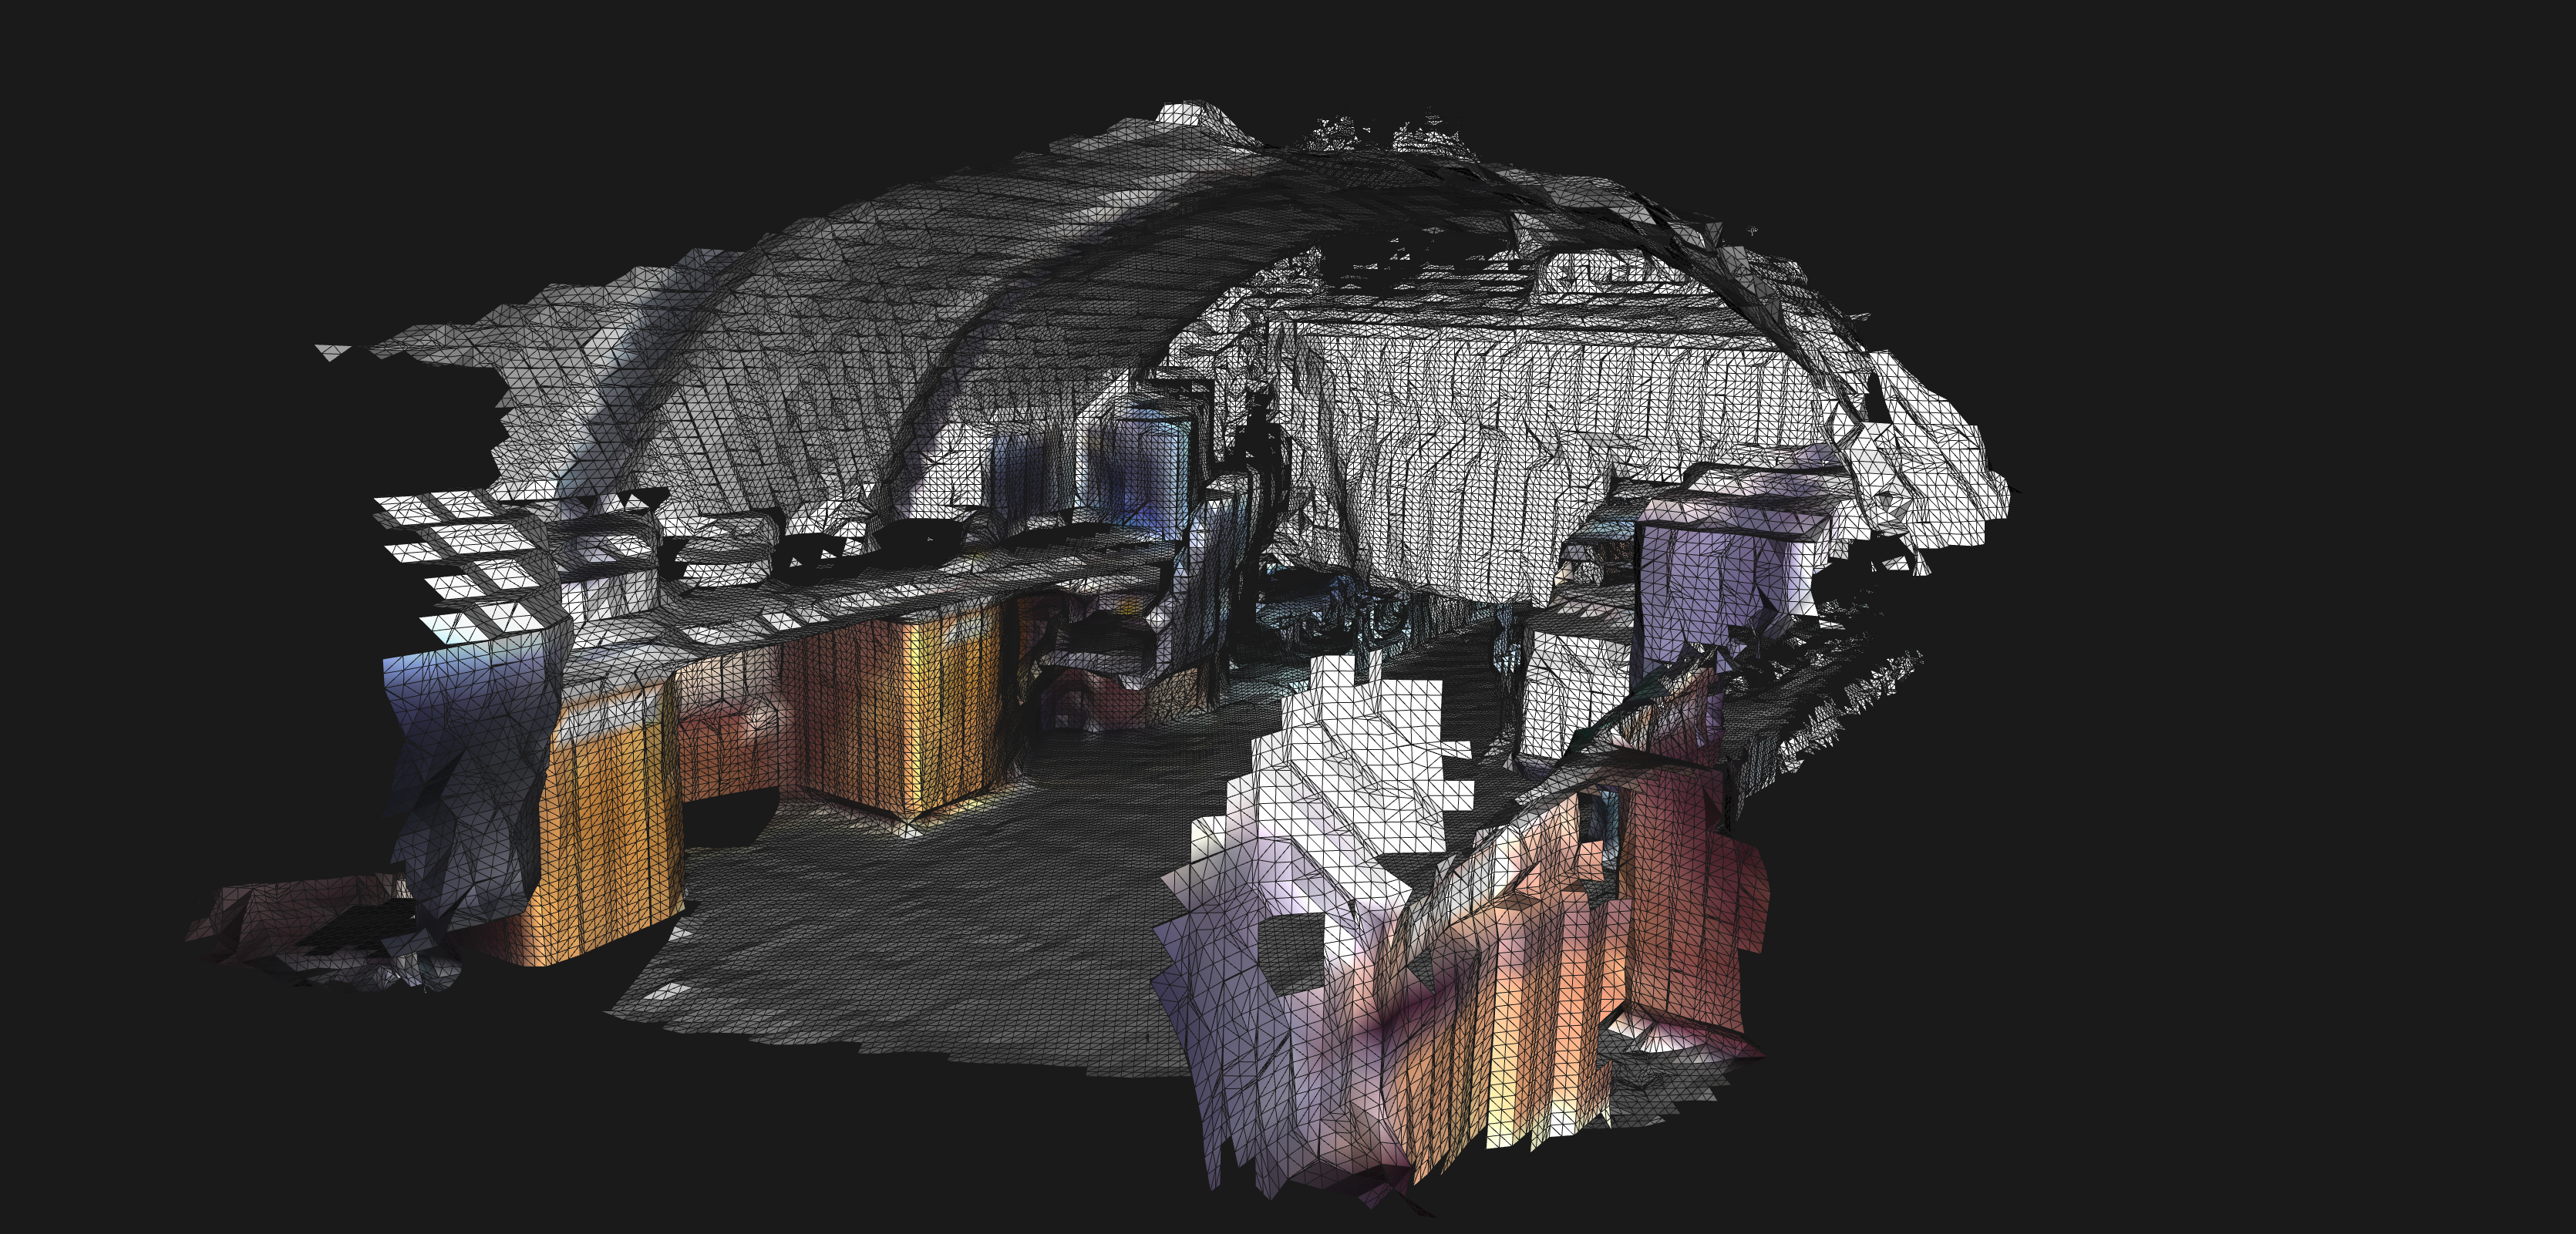
\includegraphics[width=0.8\textwidth]{mesh.png}
\caption{3D mesh reconstruction of the Fasta Robotics lab. Degraded 
geometry at center marks where a person moved during capture. The glass 
partition produces inconsistent depth returns. Both share a cause: the 
map records where surfaces were measured, not what they are.}
\label{fig:mesh}
\end{figure}

This is the map a Unitree Go2 navigated from last November. Localization 
against the arch and fixed furniture held well under fifteen centimeters. 
The failures were elsewhere. A person standing near the glass partition 
presented a compounded problem: a dynamic agent in front of a surface the 
depth sensor could not resolve. The robot had no way to separate the 
person from the partition, or the partition from the room behind it. 
It stopped.

Every surface here is encoded the same way: static, permanent, opaque. 
A relocated chair, a glass wall, a person mid-step all enter the same 
representation and receive the same treatment. This is not a sensor 
problem or a localization problem. It is structural. The map has no 
place for what a surface belongs to, whether it persists, or whether 
it can move.

The hard version of this is not labeling surfaces after the fact. It is 
building a representation where knowledge about entity type, persistence, 
and expected behavior is load-bearing: where it shapes the state estimate 
and changes how uncertainty propagates when something moves or returns no 
depth at all. That integration is largely unsolved, and it is what I want 
to work on.
\section*{When Systems Can't Adapt}

During my Master's at University of Tehran, I worked on IMU-based orientation estimation—how robots know which way is up without GPS. Traditional filters need constant retuning: parameters that work at 100Hz break at 400Hz during dynamic gaits. Calibration differences between sensors leak into estimates.

I designed a deep learning approach that treats sampling rate as an explicit input. The architecture uses 1D-CNNs for feature extraction, a bidirectional LSTM for temporal context, and a fusion layer that takes sampling rate directly before predicting orientation. Training with injected Gaussian noise made the model robust to sensor variations. Validation across 7 datasets (OxIOD, BROAD, EuRoC) covering over 200 kilometers reduced orientation error by 37\% versus EKF baselines. The model generalized across different IMUs without retraining. We published the work in \textit{Measurement} \cite{golroudbari2023imu}.

But deployment exposed the constraint. When calibration drifted—temperature changes, mechanical stress, sensor aging—predictions degraded. The model couldn't adapt online when sensor behavior changed.

I could diagnose the failure. I could see the predictions diverging from ground truth. But I couldn't fix it without retraining. The architecture I'd designed assumed sensor characteristics would stay fixed—an assumption I hadn't even realized I was making until deployment broke it. That's when I learned the difference between building something that works and understanding the assumptions that make it work. A successful paper shows a method performs well on benchmarks. A robust system needs to know when those benchmarks stop representing reality, and what to do when they do. I didn't have the formal frameworks—control theory, online learning, adaptive systems—to reason about that gap. 

\section*{When Identity Needs More Than Geometry}

At Ofogh360, I built a planogram compliance system for retail aisles: 
detect products on shelves, match them to SKUs, flag deviations. The 
constraint was severe — 204 labeled images across 53 classes. I used 
CLIP embeddings with cosine similarity matching, reaching 81\% mAP. 
What made it work was not the model but what the embedding represented: 
identity stable across viewpoint, lighting, and occlusion rather than 
appearance at a single frame.

Reading Prof. Fallon's LEXIS paper \cite{kassab2024lexis} reframed 
something I had treated as a perception problem. LEXIS uses CLIP 
embeddings for room classification, but the contribution is the 
refinement step: label propagation enforces semantic consistency across 
the map, so a room does not flicker between "kitchen" and "office" as 
lighting shifts. Individual predictions are assumed noisy. The map 
structure corrects them.

This is the same principle that makes SLAM work. A single feature match 
is unreliable; the factor graph, with constraints from many observations, 
is not. LEXIS applies that logic to semantics — but as a post-processing 
layer over a finished geometric map. The question I kept returning to was 
whether semantic observations could enter the estimation problem itself, 
not after geometry is solved but as measurements that shape it from the 
inside. That question became concrete when I returned to the warehouse problem.
\section*{When Geometry and Semantics Stay Disconnected}

At Fasta Robotics, I integrated ORB-SLAM3 with ROS2, fusing RealSense 
D435i and ZED2i stereo-depth with IMU. Localization held under 20cm 
across the full route. For human-aware navigation, I trained YOLOv12 
on 5,200 annotated warehouse frames, reaching 95\% recall at 30 FPS 
on Jetson Orin NX, and tracked people with DeepSORT. The robot avoided 
collisions. But the architecture showed its limit immediately: ORB-SLAM3 
optimized poses in 3D space while DeepSORT operated in image space, and 
the two never communicated. When someone moved behind a forklift, the 
tracker lost them. SLAM had no semantic state to predict where they 
might reappear given the 3D layout.

\begin{figure}[h]
\centering
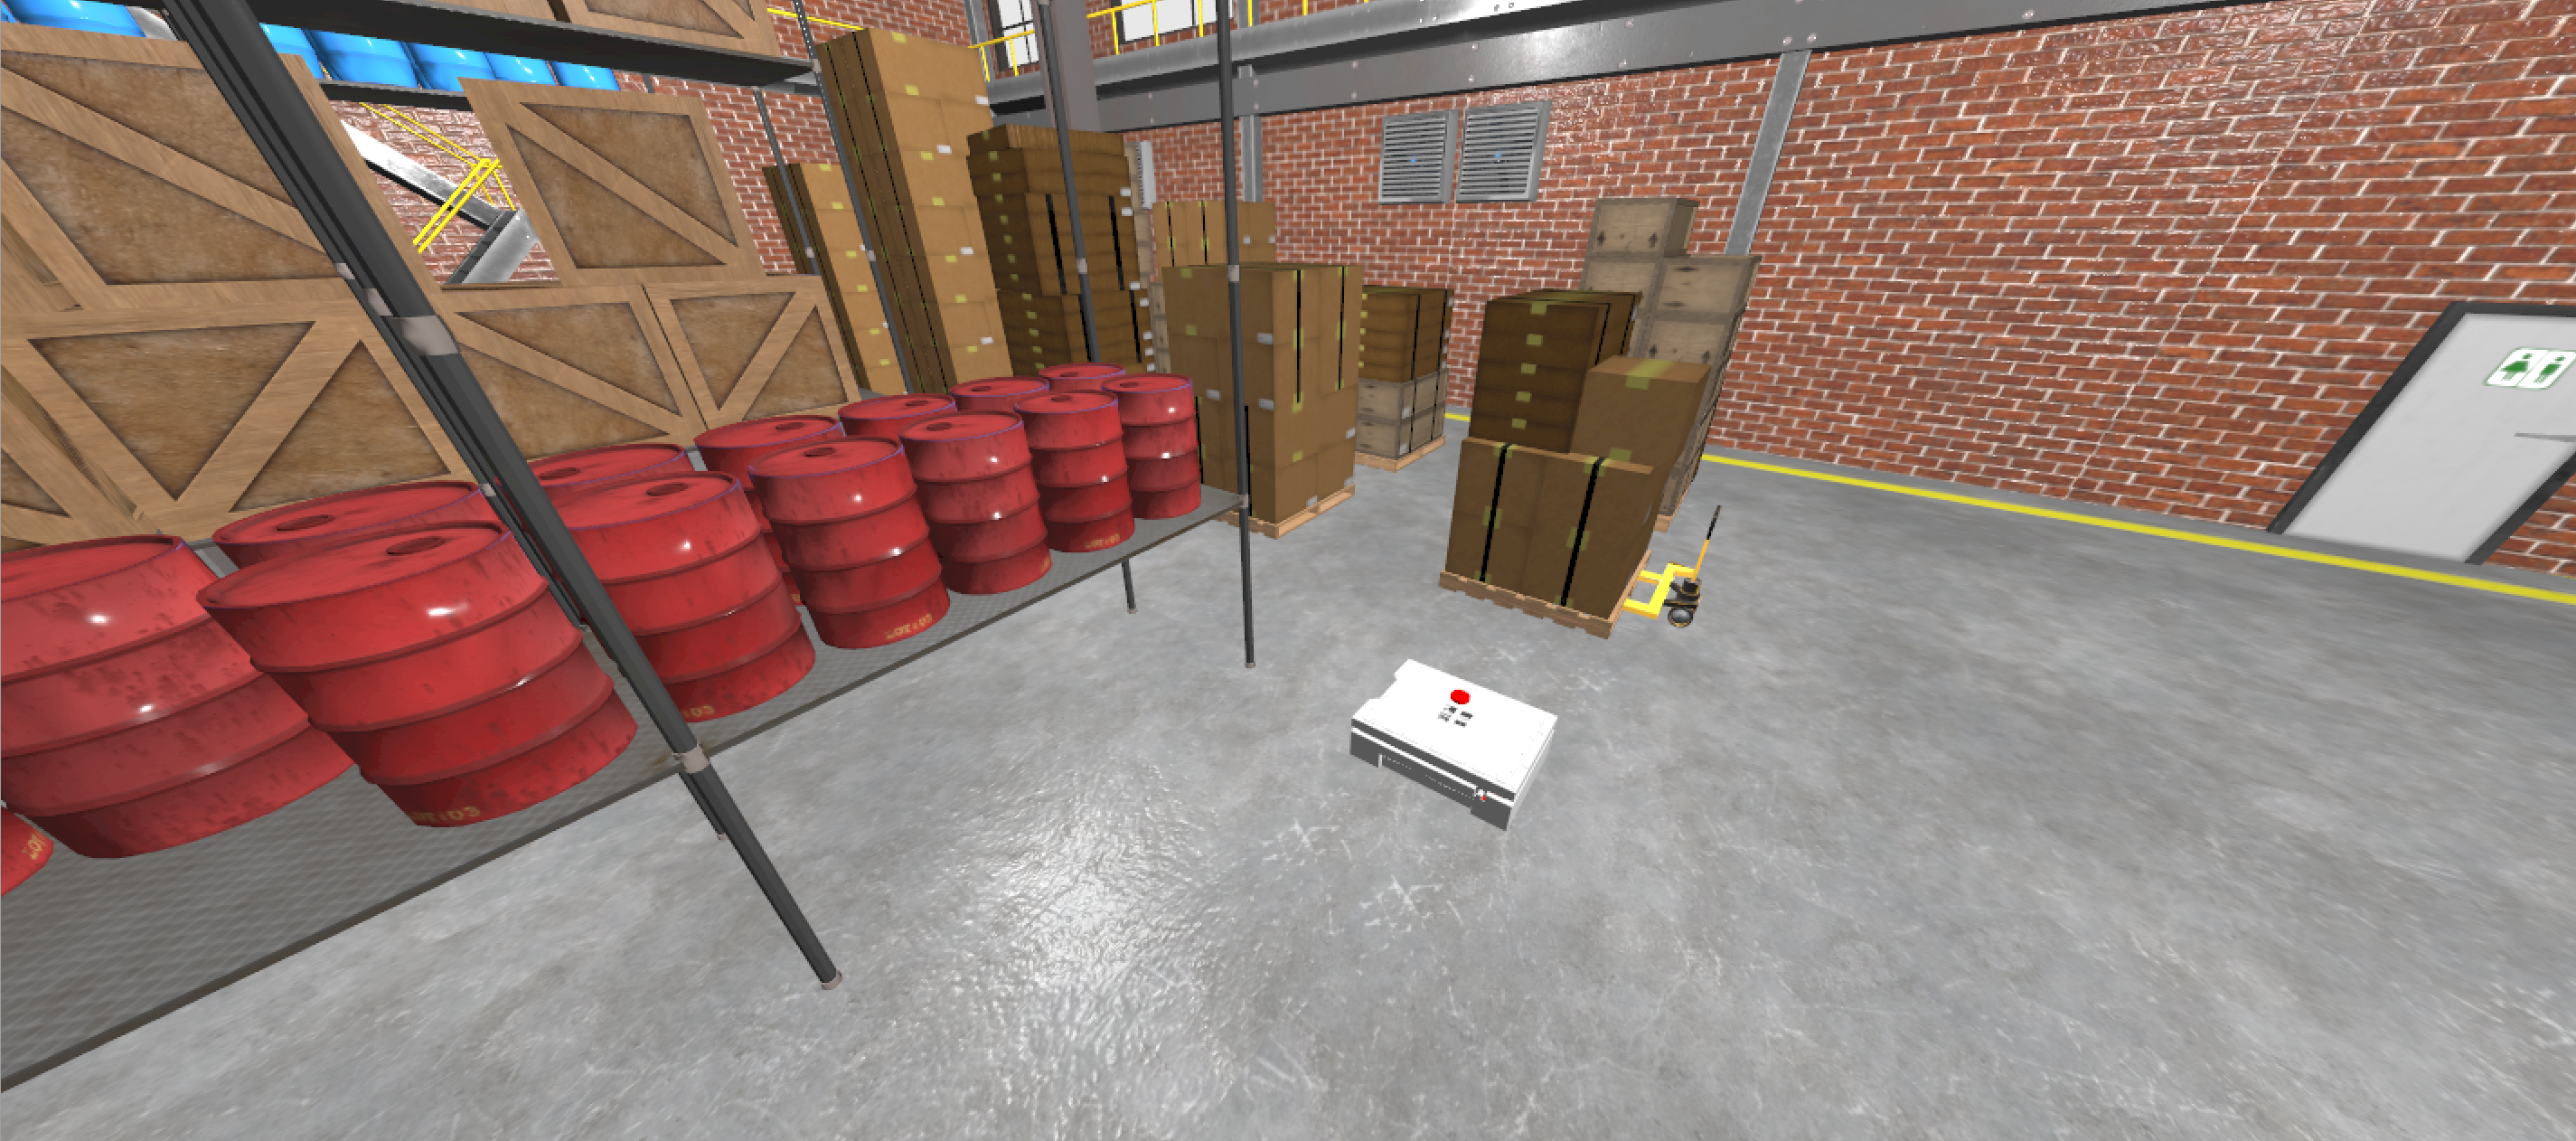
\includegraphics[width=0.8\textwidth]{warehouse.png}
\caption{Warehouse simulation environment in ROS2 and Gazebo}
\label{fig:robot}
\end{figure}

The obvious fix is to run vision-language inference continuously and 
feed it into the map. The problem is compute: on the Jetson Orin NX, 
resources are shared with locomotion and state estimation. Full 
frame-rate semantic inference is not feasible. The real question is 
whether semantic observations need to be continuous at all, or whether 
they can enter the estimation problem selectively, when geometry alone 
is insufficient.

Map structure matters here too. PlanarMesh \cite{wang2025planarmesh} 
treats reconstruction as incremental, adapting resolution so the map 
stays compact over long deployments. If semantics are to influence 
navigation persistently, the representation needs to support it: not 
a growing point cloud with frame-by-frame annotations, but structured 
geometry where stable semantic labels attach to elements that persist.

Three experiences, the same underlying constraint. The IMU work showed 
that robust systems need to model when their own assumptions break. 
The planogram work showed that the right representation matters as 
much as the algorithm. The warehouse deployment showed that 
architectural separation between geometric and semantic reasoning is 
not a detail but a fundamental limit. These were different views of 
one problem.
\section*{Adaptive Semantic-Geometric State Estimation}

The failure is not missing geometry or missing semantics — it is that 
they operate on separate tracks. Geometric estimation runs tight and 
continuous, with well-defined uncertainty. Semantic inference runs 
loosely, and its outputs have no natural place in an estimator that 
expects measurement models and covariance structure. Semantics inform 
the map after estimation is done, not during it.

Consider a legged robot re-entering a damaged building after several 
hours. Rubble has shifted, feature matching has degraded, and 
re-localization with geometric evidence alone is unreliable. Yet the 
scene is still readable at a coarser level: a stairwell, a doorframe, 
a corridor junction. The robot cannot use those cues, because it has 
no mechanism to treat a semantic observation as a constraint on pose.

Closing that gap raises four problems:

\begin{itemize}
  \item \textbf{Semantic measurement models}: A geometric factor 
  has a predicted measurement, a residual, and a covariance. 
  A VLM output has none of these. Formulating semantic observations 
  as proper factors — with calibrated uncertainty — is largely 
  unsolved.

  \item \textbf{Triggered inference}: Full frame-rate semantic 
  inference is not feasible on edge hardware. The estimator already 
  produces the signal needed to decide when semantics matter: pose 
  covariance, inlier count, loop closure confidence. Using geometric 
  uncertainty to gate inference is unexplored.

  \item \textbf{Selective retention}: Over long deployments, dense 
  semantic embeddings per surface are unsustainable. What to keep, 
  and when to retire annotations that no longer reflect the 
  environment, is an open question.

  \item \textbf{Label stability}: As meshes refine and coarsen 
  incrementally, semantic labels attached to geometric elements 
  become misaligned. Maintaining consistency through map updates, 
  without re-running inference, has no standard solution.
\end{itemize}

These are not independent. Solving them together, on real hardware, 
in environments that do not cooperate with assumptions, is what makes 
this a research problem.

\section*{Research Approach}

The core idea is to let the estimator decide when semantic inference 
runs. When pose covariance grows, feature matching degrades, or 
re-localization struggles, the system invokes semantic inference and 
the result enters as a factor with calibrated uncertainty — the same 
way a loop closure or IMU measurement does. Not a parallel pipeline 
fused afterward, but a measurement that participates in the 
optimization directly.

The work breaks into three stages. First, formulating semantic 
factors: developing uncertainty models that let vision-language 
outputs enter a factor graph alongside geometric measurements. 
Second, designing the triggering mechanism: detecting when geometric 
ambiguity is the kind semantics can resolve, not just when covariance 
is high. Third, maintaining label consistency as PlanarMesh 
\cite{wang2025planarmesh} refines and coarsens the map incrementally, 
without re-running inference on every update.

Validation will run on legged platforms in warehouse and 
damaged-building environments, where geometric cues degrade but 
semantic structure persists. The measure of success is not only 
localization accuracy, but whether semantic cues improve 
re-localization after environmental change and whether the system 
holds real-time under edge compute constraints.

\section*{Why Oxford}

Fallon's group has a specific trajectory that matters: VILENS \cite{wisth2022vilens} showed tight multi-sensor fusion in a factor graph under extreme conditions. LEXIS \cite{kassab2024lexis} added semantic understanding through vision-language models. PlanarMesh \cite{wang2025planarmesh} made reconstruction incremental and adaptive. Each piece addresses part of what I need, but they're not yet integrated. What I want to build—semantic observations as adaptive factors triggered by geometric uncertainty—requires all three foundations simultaneously.

The DRS group's infrastructure is what makes this work possible. The factor graph frameworks from VILENS give me the foundation for treating semantic observations as probabilistic measurements. The legged platforms (ANYmal, Unitree) provide the exact hardware where compute constraints and dynamic motion matter—where I need to prove semantic inference won't break real-time guarantees while the robot is walking. The group's validation environments—underground sites, damaged buildings, unstructured terrain—are where both geometric and semantic cues degrade, which is precisely when adaptive triggering should prove its value. Most importantly, the group's recent trajectory from VILENS through LEXIS to PlanarMesh shows they're already moving toward the integration I'm proposing. I'm not bringing a foreign idea to a group doing something else—I'm extending work they've already started.

Oxford is where I can build on existing infrastructure rather than starting from scratch, and where the research culture values deployment validation as much as algorithmic contribution.

But the research problem itself demands more than robotics expertise alone.

\section*{Why Autonomous Intelligent Machines and Systems}

I've built systems through implementation—IMU networks, warehouse vision, quadruped navigation. When calibration drift broke my IMU model during deployment, I diagnosed the failure but lacked formal frameworks to understand why the architecture couldn't adapt online. I can implement SLAM, but I don't have verification tools to prove semantic factors won't violate real-time guarantees when geometric uncertainty triggers inference.

Semantic SLAM sits at the intersection of AIMS's four core areas. \textbf{Robotics \& Vision} for scene understanding and state estimation. \textbf{Machine Learning} for vision-language models and their uncertainty characterization. \textbf{Control \& Verification} for real-time guarantees. \textbf{Cyber-Physical Systems} for resource-constrained deployment on legged platforms. My problem requires reasoning across all four.

The first-year training addresses the reasoning gaps I've identified. When I design triggering mechanisms for semantic inference, I need to reason about both geometric uncertainty and computational scheduling. When I formulate semantic factors, I need both probabilistic inference and real-time constraints. The interdisciplinary cohort structure matters because working alongside people tackling formal verification or security in cyber-physical networks exposes me to approaches I wouldn't encounter staying only in robotics labs.

The industrial placements close the loop. They give me direct exposure to how robotics research transitions to product—how companies evaluate whether adaptive semantic reasoning is worth the engineering cost, how they integrate research prototypes into production systems, what failure modes matter in deployment versus in papers. That's where the technical foundation I'm building meets the company I want to start. AIMS fits because it keeps both in view simultaneously: rigorous research and real-world deployment, technical depth and product thinking.

\bibliographystyle{ieeetr}
\bibliography{ref}

\end{document}
